\documentclass[12pt]{article}
\usepackage{graphicx,tikz,tikz-network,tkz-euclide}% Required for inserting images
\usepackage{amsfonts,amssymb,amsmath,float,setspace}
\title{Math Club Second Week}
\usetikzlibrary {positioning}
%\usepackage {xcolor}
\definecolor {processblue}{cmyk}{0.96,0,0,0}

\parindent 0pt
\date{October 2024}

\newcounter{problem}
\setcounter{problem}{0} % Initialize the counter at 0

\newcommand{\problem}[1]{
    \stepcounter{problem}
    \noindent\textbf{Problem \theproblem:} #1
     \\ % Add space after the problem statement
}
\newcommand{\multChoice}[5]{
    \begin{tabular}{l @{\hskip 1.5cm} l @{\hskip 1.5cm} l @{\hskip 1.5cm} l @{\hskip 1.5cm} l}
    A. #1 & B. #2 & C. #3 & D. #4 & E. #5
\end{tabular}

}
\newcommand{\solution}[1]{
    \vspace{1em} % Add space before the solution
    \noindent\textbf{Solution:} #1
     % Add space after the solution
}

\setlength{\baselineskip}{5\baselineskip}


\usetikzlibrary {positioning}
%\usepackage {xcolor}
\definecolor {processblue}{cmyk}{0.96,0,0,0}
\newcommand{\myVertex}[3]{
    \Vertex[x=#1,y=#2,size=0.5,label=$#3$,position=90,fontscale=2,style={color=blue}]{#3}
}


\begin{document}

\maketitle

 \begin{spacing}{1.3}

\section*{Problems}

\begin{problem}[C][3][AMATYC Fall 2003/10]
   % Student Math League ^ Counting
   The counting numbers are written in the pattern at
   the bottom. Find the middle number of the 40th row. 
   \begin{centering}
   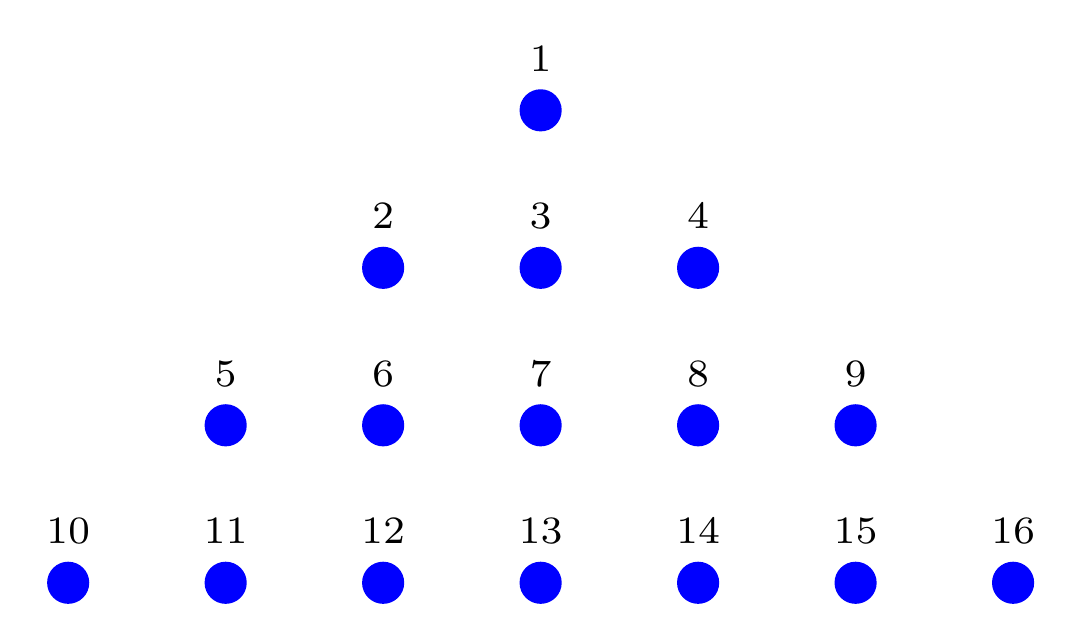
\begin{tikzpicture}
      \myVertex{9}{0}{1}
      
      \myVertex{7}{-2}{2}
      \myVertex{9}{-2}{3}
      \myVertex{11}{-2}{4}
  
      \myVertex{5}{-4}{5}
      \myVertex{7}{-4}{6}
      \myVertex{9}{-4}{7}
      \myVertex{11}{-4}{8}
      \myVertex{13}{-4}{9}
  
      \myVertex{3}{-6}{10}
      \myVertex{5}{-6}{11}
      \myVertex{7}{-6}{12}
      \myVertex{9}{-6}{13}
      \myVertex{11}{-6}{14}
      \myVertex{13}{-6}{15}
      \myVertex{15}{-6}{16}
     
  \end{tikzpicture} \vskip 0.7cm
\end{centering}
\end{problem}
\multChoice{1561}{1641}{1559}{1639}{1483}
\begin{solution}[1561]
      Notice that the last numbers of each row are $1,4,9,16,\ldots$ same as 
      $1^2,2^2,3^2,4^2,...$ , note that if we are in the $i-th$ row and it ends in $i^2$, then
      we make the next row with $2i+1$ numbers, meaning the last number of the next row is
      $i^2+2i+1=(i+1)^2$ \\
      Now, we just need to find the middle number, call it $m_i$ , here knowing the lenght of
      each row we look that $m_3=3^2-1, m_4=4^2-3$ and in the same way 
      $$m_{40}=40^2-39=1561$$
\end{solution}

\begin{problem}[N][4][AMATYC Fall 2003/2]
   % Divisibility ^ Inequalities ^ Student Math League
   A collection of coins is made up of an equal number of pennies
   , nickels, dimes, and quarters. What is the largest possible
   value of the collection which is less than \$2? \\
\end{problem}
\multChoice{\$1.64}{\$1.78}{\$1.86}{\$1.89}{\$1.99}
\begin{solution}[\$1.64]
   Since the collection is made up with an equal number of each type, it means that if it 
    has $n$ coins of each type then it has $(0.01+0.05+0.10+0.25)n=0.41n$ dollars , so we 
    have $0.41n<2 \iff n<\frac{2}{0.41}<5$ and since $n$ is a large as possible, we must 
    have $n=4$ and therefore $\$0.41\times4=\$1.64$
\end{solution}

\begin{problem}[N][2][AMATYC Fall 2003/P6]
   % Primes ^ Student Math League ^ Vieta's Formula
   Let $p$ be a prime number and $k$ an integer such that the next
    equation has two positive integer solutions for $x$
    $$ x^2 + kx + p = 0 $$

    What is the value of $k + p$? \\ 
\end{problem}
\multChoice{1}{-1}{0}{2}{-2}
\begin{solution}[B]
   Call $x_1,x_2$ to these solutions, that means
    \begin{align*}
    x^2+kx+p=&(x-x_1)(x-x_2) \\
    \iff x^2+kx+p=&x^2-(x_1+x_2)x+x_1x_2
    \end{align*}
    Since this must hold true for every $x$, then 
   \begin{align}
       p=&x_1x_2 \\
       k =& -(x_1+x_2)
   \end{align}
    (1) means that $x_1$ and $x_2$ are divisors of $p$ , and since they are positive
    and $p$ is prime, they can only be 1 and p, then using (2):
    $$k+p = -(p+1) + p = -1$$
\end{solution}


\begin{problem}[G][2][AMATYC Spring 2008/P6]
   % Pythagorean Theorem ^ Student Math League
   A circle is inscribed in a square with side length 1. What is the
    area of the region outside the circle but inside the square? \\
\end{problem}
\multChoice{1-$\pi$/4}{$\pi$/4-1}{$\pi$/4}{1-$\pi$/2}{1-$\pi$}
\begin{solution}[E]
   \begin{tikzpicture}
      % Every aspect of the figure can be altered through these definitions
      \def\radius{3} \def\X{0.35} \def\labelSpacing{1.1}
      \def\A{110} \def\B{315} \def\C{70} \def\D{215}
      
      % Restricts the canvas
      % \tkzInit[xmin=-6,xmax=6,ymin=-6,ymax=6]\tkzClip 
      \tkzDefPoints{0/0/H,8/0/T,8/8/A,0/8/M}
      \tkzDefMidPoint(T,H) \tkzGetPoint{L}
      % Find the circumcenter (intersection of bisectors)
      \tkzDefCircumCenter(M,A,L) \tkzGetPoint{O}
  
     % Draw the square
      \tkzDrawPolygon(M,A,T,H)
      \tkzDrawCircle(O,L)
      \tkzDrawPoints(M,A,T,H,L)
      \tkzDefPointBy[projection=onto A--T](O) \tkzGetPoint{R}
  
      %black points
      \tkzDrawPoints[fill=black,size=2pt](M,A,T,H,O,L,R)
      
      \tkzDrawPolygon(O,L,T,R)
      \tkzDrawSegment(O,R)
      \tkzDrawSegment[dash pattern=on 5pt off 5pt](O,A)
      \tkzLabelSegment[below](O,R){$a$}
      \tkzLabelSegment[above left](O,A){$20$}
      \tkzLabelPoints[above](M,A)
      \tkzLabelPoints[below](T,L,H){T,L,H}
      \tkzLabelPoint[above right](R){R}
      \tkzLabelPoint[above left](O){O}
   
  \end{tikzpicture}
  Let $O,L$ be the center of the circumference and the midpoint of TH respectively.
    Let $a$ be the length of LT, that is, half the size of the square
    , now let R be a point such that O,L,T,R is a rectangle, that
    means $OR=LT=a$ and $RT=OL=20$ \\
    Note that if we find $AR$ then we are done, since $AR+RT=AT=2a$, which is a side of
    the square. Then by the Pythagorean Theorem:

    \begin{align*}
        a^2+&AR^2=20^2 \\
        \iff &AR = \sqrt{20^2-a^2} 
    \end{align*}
    Finally 
     \begin{align*}
        &AR+RT=2a \\
    \iff& \sqrt{20^2-a^2} + 20 = 2a \\
    \iff& 20^2-a^2 = 2^2(a-10)^2 \\
    \iff& 5a^2-80a=0 \\
    \iff& 4a(a-16)=0 
    \end{align*}
    $a$ can't be $0$ since it's a segment, then $a=16$ and the square has length 32
\end{solution}

\begin{problem}[A][4][AMATYC Fall 2005/7]
      % System of equations ^ Student Math League
      When I am as old as my father is now, I will be five times as old as my son is now. By then, my
      son will be eight years older than I am now. The sum of my father’s age and my age is 100 years.
      How much older am I than my son? \\
\end{problem}
\multChoice{14}{16}{18}{22}{24}

\begin{solution}[D]
   Call $a,b,c$ to the ages of your father, you, and your son, then the statements are
    equivalent to say 
    \begin{align}
       a &= 5c \tag{1} \label{eq:1}\\
       c + (a-b) &= 8+b \tag{2} \label{eq:2}\\
       a+b &= 100 \tag{3} \label{eq:3}
    \end{align}
    Using $(1)$ is easy to see that
    \begin{align}
       &6c-2b = 8 \tag{I} \label{eq:I}\\
       &5c+b = 100 \tag{II} \label{eq:II}
    \end{align}

    \begin{align*}
        2(\ref{eq:II})+(\ref{eq:I}) \Rightarrow c=13,b=35 
    \end{align*}
    so you are 22 years older than your son
\end{solution}

\begin{problem}[A][3][AMATYC Fall 2008/8]
      % Analysis ^ Student Math League
      The population of Mathville grows exponentially with respect to time, and so does the number
      of car thefts. If $f(t)$ represents the number of car thefts per person in Mathville with respect to time,
      then $f(t)$ could NOT be: 
      \begin{tabular}{l r}
         A. A constant function & B. A non-constant linear function  \\
         C. an exponential growth function & D. an exponential decay function\\
         D. it could be any of these functions
         \end{tabular}
\end{problem}

\begin{solution}[B]
   Say $\mathbb{P}$ and $\mathbb{C}$ represent the population and the number of cars thefts
    with respect to time, respectively: $\mathbb{P}(t)=e^{at}$ and $\mathbb{C}(t)=e^{bt}$, 
    then we must have $f(t) = \mathbb{C}(t) / \mathbb{P}(t) = e^{(b-a)t}$.
    If $b>a$ then is C, if $a>b$ then is D and if $a=b$ then is A, since exaclty one of these statements
    must be true, $f(t)$ could not be B

\end{solution}

\begin{problem}[C][7][AMATYC Fall 2004/16]
      % Counting ^ Student Math League
      Let $A = \{0,1,2,3,4,5,6,7,8,9\}$. How many three-element subsets of A contain at least two
      consecutive integers? 
      For example if $A = \{0,1,2,3,4\}$ then
      $$  \{0,1,2\} , \{0,1,3\} , \{0,1,4\}$$ 
      $$  \{0,2,3\} , \{0,3,4\} , \{1,2,3\}$$
      $$  \{1,2,4\} , \{1,3,4\} , \{2,3,4\}$$
      are all possibilities. \\
\end{problem}
\multChoice{32}{40}{48}{56}{64}
\begin{solution}[64]
   Consider the three-element subsets of the form $\{a,a+1,b\}$ where $0\leq a \leq 7$
    for each choice of $a$ we have $8-a$ possible values of $b$, giving $1+2+...+8=36$ 
    different cases\\
    Similarly take the cases $\{b,a,a+1\}$ where $1\leq a \leq 8$ , again each choice of $a$ 
    give us $8-a$ possibilities for $b$, that is, another 36 cases.
    Now we remove the cases the cases that we double-counted, that is, the cases that 
    meet both properties, they have the form $\{a,a+1,a+2\}$ , which give us 8 cases, so
    our answer is $36+36-8=64$
\end{solution}

\end{spacing}
\end{document}
